
%% bare_jrnl_compsoc.tex
%% V1.4a
%% 2014/09/17
%% by Michael Shell
%% See:
%% http://www.michaelshell.org/
%% for current contact information.
%%
%% This is a skeleton file demonstrating the use of IEEEtran.cls
%% (requires IEEEtran.cls version 1.8a or later) with an IEEE
%% Computer Society journal paper.
%%
%% Support sites:
%% http://www.michaelshell.org/tex/ieeetran/
%% http://www.ctan.org/tex-archive/macros/latex/contrib/IEEEtran/
%% and
%% http://www.ieee.org/

%%*************************************************************************
%% Legal Notice:
%% This code is offered as-is without any warranty either expressed or
%% implied; without even the implied warranty of MERCHANTABILITY or
%% FITNESS FOR A PARTICULAR PURPOSE! 
%% User assumes all risk.
%% In no event shall IEEE or any contributor to this code be liable for
%% any damages or losses, including, but not limited to, incidental,
%% consequential, or any other damages, resulting from the use or misuse
%% of any information contained here.
%%
%% All comments are the opinions of their respective authors and are not
%% necessarily endorsed by the IEEE.
%%
%% This work is distributed under the LaTeX Project Public License (LPPL)
%% ( http://www.latex-project.org/ ) version 1.3, and may be freely used,
%% distributed and modified. A copy of the LPPL, version 1.3, is included
%% in the base LaTeX documentation of all distributions of LaTeX released
%% 2003/12/01 or later.
%% Retain all contribution notices and credits.
%% ** Modified files should be clearly indicated as such, including  **
%% ** renaming them and changing author support contact information. **
%%
%% File list of work: IEEEtran.cls, IEEEtran_HOWTO.pdf, bare_adv.tex,
%%                    bare_conf.tex, bare_jrnl.tex, bare_conf_compsoc.tex,
%%                    bare_jrnl_compsoc.tex, bare_jrnl_transmag.tex
%%*************************************************************************


% *** Authors should verify (and, if needed, correct) their LaTeX system  ***
% *** with the testflow diagnostic prior to trusting their LaTeX platform ***
% *** with production work. IEEE's font choices and paper sizes can       ***
% *** trigger bugs that do not appear when using other class files.       ***                          ***
% The testflow support page is at:
% http://www.michaelshell.org/tex/testflow/


\documentclass[10pt,conference,onecolumn,compsoc]{IEEEtran}


\usepackage{hyperref}
\usepackage{enumitem}
\setlist[itemize]{leftmargin=3 cm}
\setlist[enumerate]{leftmargin=3cm}



% *** CITATION PACKAGES ***
%
\ifCLASSOPTIONcompsoc
  % IEEE Computer Society needs nocompress option
  % requires cite.sty v4.0 or later (November 2003)
  \usepackage[nocompress]{cite}
\else
  % normal IEEE
  \usepackage{cite}
\fi
% cite.sty was written by Donald Arseneau
% V1.6 and later of IEEEtran pre-defines the format of the cite.sty package
% \cite{} output to follow that of IEEE. Loading the cite package will
% result in citation numbers being automatically sorted and properly
% "compressed/ranged". e.g., [1], [9], [2], [7], [5], [6] without using
% cite.sty will become [1], [2], [5]--[7], [9] using cite.sty. cite.sty's
% \cite will automatically add leading space, if needed. Use cite.sty's
% noadjust option (cite.sty V3.8 and later) if you want to turn this off
% such as if a citation ever needs to be enclosed in parenthesis.
% cite.sty is already installed on most LaTeX systems. Be sure and use
% version 5.0 (2009-03-20) and later if using hyperref.sty.
% The latest version can be obtained at:
% http://www.ctan.org/tex-archive/macros/latex/contrib/cite/
% The documentation is contained in the cite.sty file itself.



% *** GRAPHICS RELATED PACKAGES ***
%
\ifCLASSINFOpdf
   \usepackage[pdftex]{graphicx}
 
\else
 
\fi
% graphicx was written by David Carlisle and Sebastian Rahtz. It is
% required if you want graphics, photos, etc. graphicx.sty is already
% installed on most LaTeX systems. The latest version and documentation
% can be obtained at: 
% http://www.ctan.org/tex-archive/macros/latex/required/graphics/
% Another good source of documentation is "Using Imported Graphics in
% LaTeX2e" by Keith Reckdahl which can be found at:
% http://www.ctan.org/tex-archive/info/epslatex/
%
% latex, and pdflatex in dvi mode, support graphics in encapsulated
% postscript (.eps) format. pdflatex in pdf mode supports graphics
% in .pdf, .jpeg, .png and .mps (metapost) formats. Users should ensure
% that all non-photo figures use a vector format (.eps, .pdf, .mps) and
% not a bitmapped formats (.jpeg, .png). IEEE frowns on bitmapped formats
% which can result in "jaggedy"/blurry rendering of lines and letters as
% well as large increases in file sizes.
%
% You can find documentation about the pdfTeX application at:
% http://www.tug.org/applications/pdftex









% *** PDF, URL AND HYPERLINK PACKAGES ***
%
\usepackage{url}
% url.sty was written by Donald Arseneau. It provides better support for
% handling and breaking URLs. url.sty is already installed on most LaTeX
% systems. The latest version and documentation can be obtained at:
% http://www.ctan.org/tex-archive/macros/latex/contrib/url/
% Basically, \url{my_url_here}.




\begin{document}

\title{Temtris}
%
%

% received ..."  text while in non-compsoc journals this is reversed. Sigh.

\author{Curt Lynch and Hunter Johnson}

\IEEEtitleabstractindextext{%
\begin{abstract}
Temtris is a Tetris-like we are developing as part of our CSCI352 class.
\end{abstract}
}

% make the title area
\maketitle

\IEEEdisplaynontitleabstractindextext

\IEEEpeerreviewmaketitle

\section{Introduction}
Temtris is a wpf application that we aim to be Tetris clone. Tetris, is a game where 4 block section shapes fall from top down and you try to fit rows of these blocks together at an ever increasing pace until the screen inevitably fills causing game over. A score is computed based on how efficiently you clear the board as the game progresses, with more points being awarded for streaks of row clears and tetris row clears. Temtris will include this regular mode with it's locked shape patterns, as well as a mode where the blocks are randomly generated within certain parameters. Our target audience would probably be the select few who call themselves "gamers", as well as those who are looking for a casual way to pass the time. We are making Temtris as a duo as part of our CSCI 352 class. That being the case, we still want Temtris to be a fun and interesting game for anyone looking to play.

\subsection{Background}
A Tetrimino is one of the 7 classic Tetris shapes; these include the O, I, T, L, J, S, and Z shapes. Each Tetrimino is made up of four squares called minos. The matrix is the space where the Tetris game is played. A 'line clear' happens when a horizontal row is completely filled, causing it to be removed from the matrix. Lock-down is when a Tetrimino is locked into its current position and is no longer controllable.

Also, consider going into your personal connection with this project -- why did you decide to do it?
Whilst attempting to come up with ideas, the idea of remaking Tetris came up, and to clarify this is coming from Hunter, when I heard Tetris my brain went full monkey, "ooh ooh ahh ahh Tetris funny, seems more interesting than anything else we have thought up" and that's how we landed on Temtris.  

\subsection{Impacts}
Temtris is a great way to improve our skills and better prepare us for working on more impactful projects in the future. Impact wise, towards the greater scale of coding, it has none, but for personal entertainment as well as great c\# practice it will be quite impactfull. 

\subsection{Challenges}
This is the first moderately sized project either of us has attempted. This is also our first real foray into WPF and c\# so there are some growing pains there as well. As for the project itself, I suspect getting the movement and rotations to feel like a proper Tetris game will take much more fine tuning than we have needed to use in the past.

\section{Scope}
Our initial goal is to implement the following typical parts of a Tetris-like: 
\begin{itemize}
\item Implement a main menu with access to settings and game modes.
\item Have controllable tetriminos that fall into place in the matrix.
\item Implement all 7 tetrimino variants. 
\item Have rows that disappear when they fill up, i.e., the line clears.
\item Keep score or track how well the player does in some way.
\item Display the next piece to spawn.
\item Play background music and have sound effects for line clears, player actions, etc.
\end{itemize}

For stretch goals, we would like to add the following:
\begin{itemize}
\item Implement a multiplayer mode. Having at least two clients with a competitive game mode over LAN or just sharing a keyboard.
\item Different power-ups may be earned by removing a certain amount of one color from the board.
\end{itemize}

\subsection{Requirements}
As part of fleshing out the scope of your requirements, you'll also need to keep in mind both your functional and non-functional requirements.  These should be listed, and explained in detail as necessary.  Use this area to explain how you gathered these requirements.

\subsubsection{Functional}
\begin{itemize}
\item User needs to have a private shopping cart -- this cannot be shared between users, and needs to maintain state across subsequent visits to the site
\item Users need to have website accounts -- this will help track recent purchases, keep shopping cart records, etc.
\item You'll need more than 2 of these...
\end{itemize}

\subsubsection{Non-Functional}
\begin{itemize}
\item Security -- user credentials must be encrypted on disk, users should be able to reset their passwords if forgotten
\item you'll typically have fewer non-functional than functional requirements
\end{itemize}

\subsection{Use Cases}
This subsection is arguably part of how you define your project scope (why it is in the Scope section...).  In a traditional Waterfall approach, as part of your requirements gathering phase (what does the product actually \emph{need} to do?), you will typically sit down with a user to develop use cases.

You should have a table listing all use cases discussed in the document, the ID is just the order it is listed in, the name should be indicative of what should happen, the primary actor is typically most important in an application where you may have different levels of users (think admin vs normal user), complexity is a best-guess on your part as to how hard it should be.  A lower number in priority indicates that it needs to happen sooner rather than later.  A sample table, or Use Case Index can be seen in Table \ref{tab:useCaseIndex}.




\begin{table}
\centering
\begin{tabular}{|c|c|c|c|c|}
\hline
Use Case ID & Use Case Name & Primary Actor & Complexity & Priority \\
\hline \hline
1 & Add item to cart & Shopper & Med & 1\\
\hline
2 & Checkout & Shopper & Med & 1\\
\hline

\end{tabular}
\caption{Sample use case table}
\label{tab:useCaseIndex}
\end{table}


\begin{itemize}
\item[Use Case Number:] 1
\item[Use Case Name:] Add item to cart
\item[Description:] A shopper on our site has identified an item they wish to buy.  They will click on a ``Add to Cart" button.  This will kick off a process to add one instance of the item to their cart.
\end{itemize}

You will then go on to (minimally) discuss a basic flow for the process:

\begin{enumerate}
\item User navigates to page listing desired item
\item User left-clicks on ``Add to Cart" button.
\item User cart is updated to reflect the new item, this also updates the current total.
\item[Termination Outcome:] The user now has a single instance of the item in their cart.
\end{enumerate}

You may need to also add in any alternative flows:

Alternative: Item already exists in the cart
\begin{enumerate}
\item User navigates to page listing desired item
\item User left-clicks on ``Add to Cart" button.
\item User cart is updated to reflect the new item, showing that one more instance of the existing item has been added.  This also updates the current total.
\item[Termination Outcome:] The user now has multiple instances of the item in their cart.
\end{enumerate}

You will often also need to include pictures or diagrams.  It is quite common to see use-case diagrams in such write-ups.  To properly reference an image, you will need to use the \texttt{figure} environment and will need to reference it in your text (via the \texttt{ref} command) (see Figure \ref{cat1}).  NOTE: this is not a use case diagram, but a kitten.

After fully describing a use case, it is time to move on to the next use case:

\begin{itemize}
\item[Use Case Number:] 2
\item[Use Case Name:] Checkout
\item[Description:] A shopper on our site has finished shopping.  They will click on a ``Checkout" button.  This will kick off a process to calculate cart total, any taxes, shipping rates, and collect payment from the shopper.

\end{itemize}

You will then need to continue to flesh out all use cases you have identified for your project.

\begin{figure}[ht!]
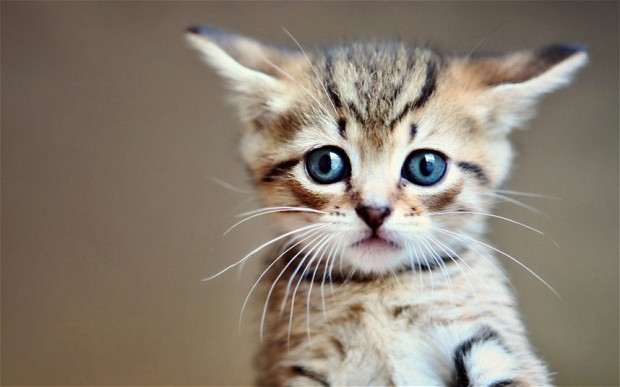
\includegraphics[height=250px, width=350px]{cat1.jpg}
\caption{First picture, this is a kitten, not a use case diagram}
\label{cat1}
\end{figure}

\subsection{Interface Mockups}
At first, this will largely be completely made up, as you get further along in your project, and closer to a final product, this will typically become simple screenshots of your running application.

In this subsection, you will be showing what the screen should look like as the user moves through various use cases (make sure to tie the interface mockups back to the specific use cases they illustrate).



\section{Project Timeline}
Go back to your notes and look up a typical project development life cycle for the Waterfall approach.  How will you follow this life cycle over the remainder of this semester?  This will usually involve a chart showing your proposed timeline, with specific milestones plotted out.  Make sure you have deliverable dates from the course schedule listed, with a plan to meet them (NOTE: these are generally optimistic deadlines).

\section{Project Structure}
At first, this will be a little empty (it will need to be filled in by the time you turn in your final report).  This is your chance to discuss all of your design decisions (consider this the README's big brother).

\subsection{UML Outline}
Show the full structure of your program.  Make sure to keep on updating this section as your project evolves (you often start out with one plan, but end up modifying things as you move along).  As a note, while Dia fails miserably at generating pdfs (probably my fault), I have had much success with png files.  Make sure to wrap your images in a \texttt{figure} environment, and to reference with the \texttt{ref} command.  For example, see Figure \ref{cat2}.

\begin{figure}[ht!]
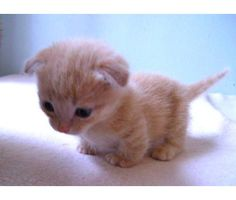
\includegraphics[scale=1.5]{cat2.jpg}
\caption{Your figures should be in the \emph{figure} environment, and have captions.  Should also be of diagrams pertaining to your project, not random internet kittens}
\label{cat2}
\end{figure}


\subsection{Design Patterns Used}
Make sure to actually use at least 2 design patterns from this class.  This is not normally part of such documentation, but largely just specific to this class -- I want to see you use the patterns!


\section{Results}
This section will start out a little vague, but it should grow as your project evolves.  With each deliverable you hand in, give me a final summary of where your project stands.  By the end, this should be a reflective section discussing how many of your original goals you managed to attain/how many desired use cases you implemented/how many extra features you added.

\subsection{Future Work}
Where are you going next with your project?
For early deliverables, what are your next steps?  (HINT: you will typically want to look back at your timeline and evaluate: did you meet your expected goals?  Are you ahead of schedule?  Did you decide to shift gears and implement a new feature?)
By the end, what do you plan on doing with this project?  Will you try to sell it?  Set it on fire?  Link to it on your resume and forget it exists?




\begin{thebibliography}{1}

\bibitem{IEEEhowto:kopka}
H.~Kopka and P.~W. Daly, \emph{A Guide to \LaTeX}, 3rd~ed.\hskip 1em plus
  0.5em minus 0.4em\relax Harlow, England: Addison-Wesley, 1999.

\end{thebibliography}



\begin{IEEEbiography}{Michael Shell}
Biography text here.
\end{IEEEbiography}

% if you will not have a photo at all:
\begin{IEEEbiographynophoto}{John Doe}
Biography text here.
\end{IEEEbiographynophoto}

% insert where needed to balance the two columns on the last page with
% biographies
%\newpage

\begin{IEEEbiographynophoto}{Jane Doe}
Biography text here.
\end{IEEEbiographynophoto}





% that's all folks
\end{document}


